\chapter{The Standard Model}

\section{Overview}

\textit{A} Standard Model is another name for a theory of the internal symmetry group $SU(3)_C \otimes SU(2)_L \otimes U(1)_Y$, with its associated set of parameters.
\textit{The} Standard Model refers specifically to a Standard Model with the proper parameters to describe the universe.
The SM is the culmination of years of work in both theoretical and experimental particle physics.  \todo{cite}
In this thesis, we take the view that theorists construct a model with the field content and symmetries as inputs, and write down the most general Lagrangian consistent with those symmetries.
Assuming this model is compatible with nature (in particular, the predictions of the model are consistent with previous experiments), experimentalists are responsible measuring the parameters of this model
This will be applicable for this chapter and the following one.

Additional theoretical background is in \ref{app:qft_symmetries}.
The philosophy and notations are inspired by \cite{yuvalSMLectures, Buchmuller:984122}.

\section{Field Content}\label{sec:field_content}

The Standard Model field content is
\begin{align}
\text{Fermions }       &:  Q_L(3,2)_{+1/3}, \xspace  U_R(3,1)_{+4/3},\xspace  D_R(3,1)_{-2/3} ,\xspace  L_L(1,2)_{-1} ,\xspace  E_R(1,1)_{-2} \notag \\
\text{Scalar (Higgs) } &:  \phi(1,2)_{+1} \\
\text{Vector Fields }  &:  G^\mu(8,1)_0 , \xspace W^\mu(1,3)_0 , \xspace B^\mu(1,1)_0 \notag
\end{align}
where the $(A, B)_Y$ notation represents the irreducible representation under $SU(3)$ and $SU(2)$, with $Y$ being the electroweak hypercharge.
Each of these fermion fields has an additional index, representing the three generation of fermions.

We observed that $Q_L, U_R,$ and $D_R$ are triplets under $SU(3)_C$; these are the \textit{quark} fields.
The \textit{color} group, $SU(3)_C$ is mediated by the \textit{gluon} field $G^\mu(8,1)_0$, which has 8 degrees of freedom.
The fermion fields $L_L(1,2)_{-1}$ and $  E_R(1,1)_{-2} $ are singlets under $SU(3)_C$; we call them the \textit{lepton} fields.

Next, we note the ``left-handed'' (``right-handed'') fermion fields, denoted by $L$ ($R$) subscript,
The left-handed fields form doublets under $SU(2)_L$.
These are mediated by the three degrees of freedom of the  ``W'' fields $W^\mu(1,3)_0$.
These fields only act on the left-handed particles of the Standard Model.
This is the reflection of the ``chirality'' of the Standard Model; the left-handed and right-handed particles are treated differently by the electroweak forces.
The right-handed fields, $U_R, D_R$, and $E_R$, are singlets under $SU(2)_L$.

The $U(1)_Y$ symmetry is associated to the $B^\mu(1,1)_0$ boson with one degree of freedom.
The charge $Y$ is known as the electroweak hypercharge.

To better understand the phenomenology of the Standard Model, let us investigate each of the \textit{sectors} of the Standard Model separately.

\subsection{Electroweak sector}

The electroweak sector refers to the $SU(2)_L \otimes U(1)_Y$ portion of the Standard Model gauge group.
Following our philosophy of writing all gauge-invariant and renormalizable terms, the electroweak Lagrangian can be written as
\begin{equation}\label{eq:ew_lagr}
\Lagr =  W^{\mu\nu}_a W_{\mu\nu}^a + B^{\mu\nu} B_{\mu\nu} + (\Dmuup \phi)^\dagger \Dmu \phi -  \mu^2 \phi^\dagger \phi - \lambda (\phi^\dagger \phi)^2.
\end{equation}
where $W^{\mu\nu}_a$ are the three ($a=1,2,3$) gauge bosons associated to the $SU(2)_L$ gauge group, $B^{\mu\nu}$ is the one gauge boson of the $U(1)_Y$ gauge group, and $\phi$ is the complex Higgs multiplet.
The covariant derivative $\Dmuup$ is given by
\begin{equation}
\Dmuup = \dmuup  + \frac{ig}{2} W^\mu_a \sigma_a + \frac{i g'}{2} B^\mu
\end{equation}
where $i \sigma_a$ are the Pauli matrices times the imaginary constant, which are the generators for $SU(2)_L$, and $g$ and $g'$ are the $SU(2)_L$ and $U(1)_Y$ coupling constants, respectively.
The field strength tensors  $W^{\mu\nu}_a$ and $B^{\mu\nu}$ are given by the commutator of the covariant derivative associated to each field
\begin{align} \label{eq:ew_field_strength_tensor}
B^{\mu\nu}   &=  \dmuup B^\nu - \partial^\nu B^\mu & \\
W^{\mu\nu}_a &=  \dmuup W^\nu_a - \partial^\nu W^\mu_a - g \epsilon_{abc} W^\mu_a W^\nu_b,& i = 1,2,3 \notag
\end{align}
\begin{figure}
\caption{Sombrero potential}
\label{fig:sombrero}
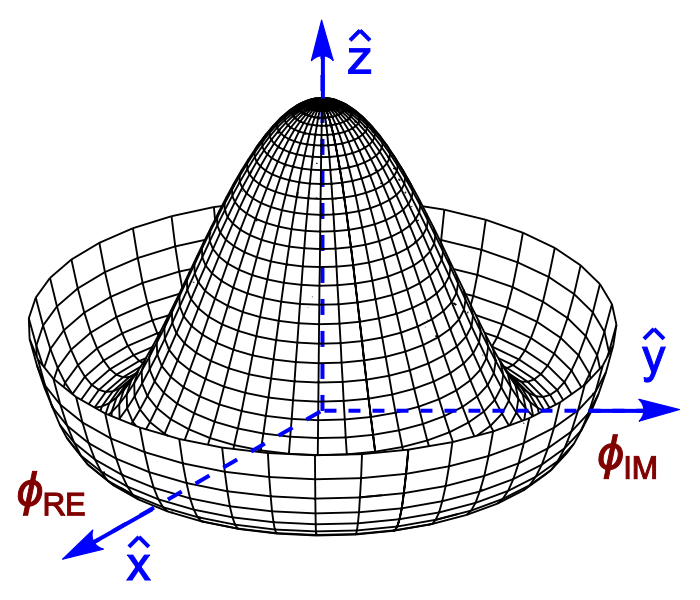
\includegraphics[width=.9\linewidth]{sombrero_potential}
\end{figure}

The terms in the Lagrangian \ref{eq:ew_lagr} proportional to $\mu^2$ and $\lambda$ make up the ``Higgs potential'' \cite{Higgs:1964pj}.
As normal (see Appendix \ref{app:qft_symmetries}), we restrict $\lambda > 0$ to guarantee our potential is bounded from below, and we also require $\mu^2 < 0$, which gives us the standard ``sombrero'' potential shown in \ref{fig:sombrero}.

This potential has infinitely many minima at $<\phi> = \sqrt{2m/\lambda}$; the ground state is \textit{spontaneously} broken by the choice of ground state, which induces a vacuum expection value (VEV).
Without loss of generality, we can choose the Higgs field $\phi$ to point in the real direction, and write the Higgs field $\phi$ in the following form :
\begin{equation}
\phi = \frac{1}{\sqrt{2}} \exp( \frac{i}{v} \sigma_a \theta_a ) \begin{pmatrix} 0 \\ v + h(x) \end{pmatrix}.
\end{equation}
We choose a gauge to rotate away the dependence on $\theta_a$, such that we can write simply
\begin{equation}
\label{eq:higgs_field_after_ssb}
\phi = \frac{1}{\sqrt{2}} \begin{pmatrix} 0 \\ v + h(x) \end{pmatrix}.
\end{equation}
Now, we can see how the masses of the vector bosons are generated from the application of the Higgs mechanism.
We plug Eq.\ref{eq:higgs_field_after_ssb} back into the electroweak Lagrangian, and only showing the relevant mass terms in the vacuum state where $h(x) = 0$  see that (dropping the Lorentz indices) :
\begin{align}
\Lagr_M = \frac{1}{8} \begin{vmatrix} \begin{pmatrix} gW_3 + g'B & g(W_1 - iW_2)\\ g(W_1 + iW_2) & -gW_3 + g'B \end{pmatrix}  \begin{pmatrix} 0  \\ v \end{pmatrix} \end{vmatrix}^2\\ = \frac{g^2 v^2}{8} \begin{bmatrix} W_1^2 + W_2^2 + (\frac{g'}{g}B - W_3)^2 \end{bmatrix} \notag
\end{align}
Defining the \textit{Weinberg} angle $\tan(\theta_W) = g'/g$ and the following \textit{physical} fields :
\begin{align}
W^{\pm} &= \frac{1}{\sqrt{2}}(W_1 \mp iW_2) \\
Z^0 &= \cos \theta_W W_3 - \sin\theta_W B \notag\\
A^0 &= \sin \theta_W W_3 + \cos\theta_W B \notag
\end{align}
we can write the piece of the Lagrangian associated to the vector boson masses as
\begin{equation}
\Lagr_{M_V} = \frac{1}{4} g^2 v^2 W^+ W^- + \frac{1}{8} (g^2 + g'^2)v^2 Z^0 Z^0 .
\end{equation}
and we have the following values of the masses for the vector bosons :
\begin{align}
m_W^2 &= \frac{1}{4}  v^2 g^2  \\
m_Z^2 &= \frac{1}{4}  v^2 (g^2 + g'^2)  \notag \\
m_A^2 &= 0  \notag
\end{align}
We thus see how the Higgs mechnanism gives rise to the masses of the $W^{\pm}$ and $Z$ boson in the Standard Model; the mass of the photon is zero, as expected.
The $SU(2)_L \otimes U(1)_Y$ symmetry of the initially massless $W_{1,2,3}$ and $B$ fields is broken to the $U(1)_{EM}$.
Of the four degrees of freedom in the complex Higgs doublet, three are ``eaten'' when we give mass to the $W^\pm$ and $Z_0$, while the other degree of freedom is the Higgs particle, as found in 2012 by the ATLAS and CMS collaborations \cite{HIGG-2012-27, CMS-HIG-12-028}.

\subsection{Quantum Chromodynamics}

Quantum chromodynamics (or the theory of the \textit{strong} force) characterizes the behavior of \textit{colored} particles, collectively known as \textit{partons}.
The partons of the Standard Model are the (fermionic) quarks, and the (bosonic) gluons.
The strong force is governed by $SU(3)_C$, an unbroken symmetry in the Standard Model, which implies the gluon remains massless.
Defining the covariant derivative for QCD as
\begin{align}
\Dmuup = \dmuup + ig_s G^\mu_a L_a, a = 1,...,8
\end{align}
where $L_a$ are the generators of $SU(3)_C$, and $g_s$ is the coupling constant of the strong force.
The QCD Lagrangian then is given by
\begin{equation}
\Lagr_{\text{QCD}} = i \bar{\psi}_f \Dmu \gamma^\mu \psi_f - \frac{1}{4} G_{a,\mu\nu} G_a^{\mu\nu}
\end{equation}
where the summation over $f$ is for quarks \textit{families}, and $ G_a^{\mu\nu}$ is the gluon field strength tensor, given by
\begin{equation}
G^{\mu\nu}_a = \dmuup G^\nu_a - \partial^\nu G^\mu_a - g_s f^{abc} G^\mu_b G^\nu_c, a,b,c = 1,...,8
\end{equation}
where $f^{abc}$ are the structure constants of $SU(3)_C$, which are analogous to $\epsilon_{abc}$ for $SU(2)_L$.
The kinetic term for the quarks is contained in the standard $\dmu$ term, while the field strength term contains the interactions between the quarks and gluons, as well as the gluon self-interactions.

Written down in this simple form, the QCD Lagrangian does not seem much different from the QED Lagrangian, with the proper adjustments for the different group structures.
The gluon is massless, like the photon, so one could n\"aively expect an infinite range force, and it pays to understand why this is not the case.
The reason for this fundamental difference is the gluon self-interactions  arising in the field strength tensor term of the Lagrangian.
This leads to the phenomena of \textit{color confinement}, which describes how one only observes color-neutral particles alone in nature.
In contrast to the electromagnetic force, particles which interact via the strong force experience a \textit{greater} force as the distance between the particles increases.
At long distances, the potential is given by $V(r) = -kr$.
At some point, it is more energetically favorable to create additional partons out of the vacuum than continue pulling apart the existing partons, and the colored particles undergo \textit{fragmentation}.
This leads to \textit{hadronization}.
Bare quarks and gluons are actually observed as sprays of hadrons (primarly kaons and pions); these sprays are known as \textit{jets}, which are what are observed by experiments.

\begin{figure}
\caption{Cross-sections of various Standard Model processes}
\label{fig:sm_xsec}
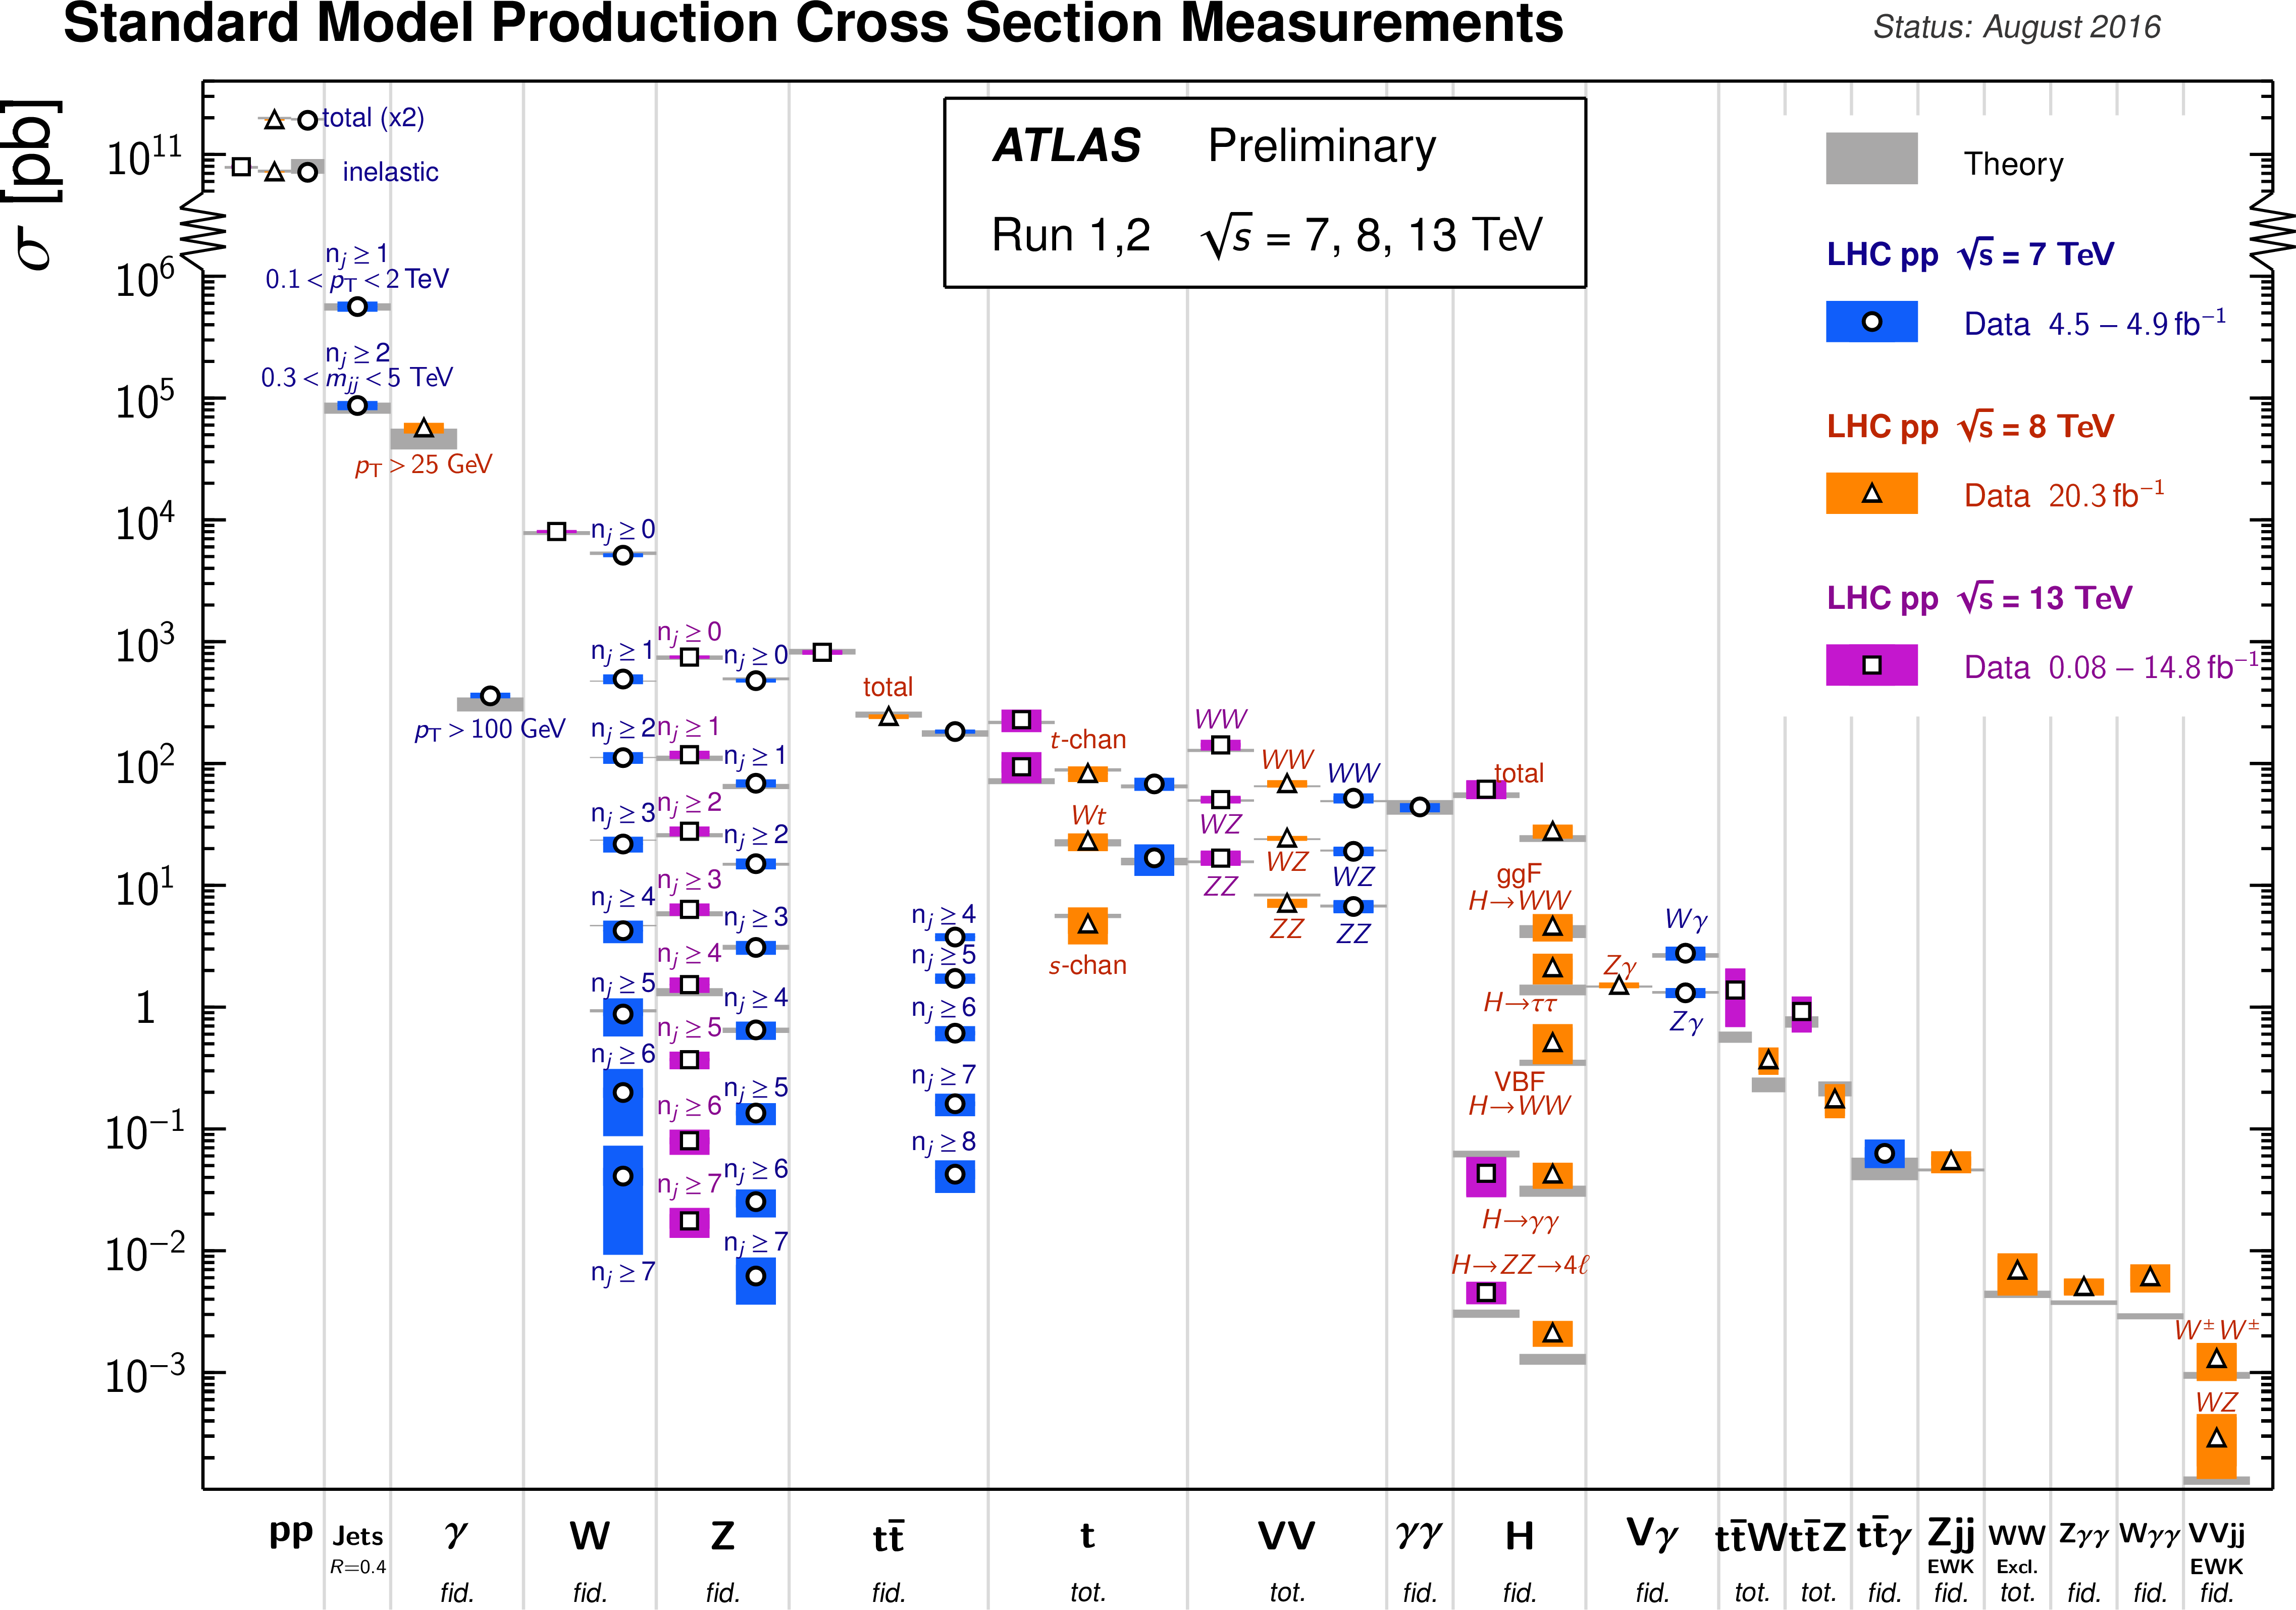
\includegraphics[width=.9\linewidth]{ATLAS_b_SMSummary_FiducialXsect}
\end{figure}

It is important to recognize the importance of understanding these QCD interactions in high-energy hadron colliders such as the LHC.
Since protons are hadrons, proton-proton collisions such as those produced by the LHC are primarily governed by the processes of QCD.
In particular, by far the most frequent process observed in LHC experiments is dijet production from gluon-gluon interactions (see Fig.\ref{fig:sm_xsec}).
These gluons that interact are part of the \textit{sea} particles inside the proton; the simple $p = uud$ model does not apply.
The main \textit{valence} $uud$ quarks are constantly interacting via gluons, which can themselves radiate gluons or split into quarks, and so on.
A more useful understanding is given by the colloquially-known \textit{bag} model \cite{Chodos:1974je, Chodos:1974pn}, where the proton is seen as a ``bag'' of (in principle) infinitely many partons, each with energy $ E < \sqrt{s} = 6.5 \TeV$.
One then collides this (proton) bag with another, and views the products of this very complicated collision, where calculations include many loops in nonpertubative QCD calculations.

Fortunately, we are generally saved by the QCD factorization theorems \cite{Collins:1989gx}.
This allows one to understand the hard (i.e. short distance or high energy) $2 \rightarrow 2$ parton process using the tools of perturbative QCD, while making series of approximations known as a \textit{parton shower} model to understand the additional corrections from nonpertubative QCD.
We will discuss the reconstruction of jets by experiments in Ch.\ref{Chapter-ATLAS}.

\subsection{Fermions}

We will now look more closely at the fermions in the Standard Model \cite{Agashe:2014kda}.

As noted earlier in Sec.\ref{sec:field_content}, the fermions of the Standard Model can be first distinguished between those that interact via the strong force (quarks) and those which do not (leptons).

There are six leptons in the Standard Model, which can be placed into three \textit{generations}.
\begin{equation}
\begin{pmatrix} e \\ \nu_e \end{pmatrix} , \begin{pmatrix} \mu \\ \nu_\mu \end{pmatrix}, \begin{pmatrix} \tau \\ \nu_\tau \end{pmatrix}
\end{equation}
There is the electron ($e)$, muon ($\mu$), and tau ($\tau$), each of which has an associated neutrino ($\nu_e, \nu_\mu, \nu_\tau$).
Each of the so-called charged (``electron-like'') leptons has electromagnetic charge $-1$, while the neutrinos all have $q_{EM} = 0$.

Often in an experimental context, lepton is used to denote the stable electron and metastable muon, due to their striking experimental signatures.
Taus are often treated separately, due to their much shorter lifetime of $\tau_{\tau} \order 10^{-13} s$; these decay through hadrons or the other leptons, so often physics analyses at the LHC treat them as jets or leptons, as will be done in this thesis.

As the neutrinos are electrically neutral, nearly massless, and only interact via the weak force, it is quite difficult to observe them directly.
Since LHC experiments rely overwhelmingly on electromagnetic interactions to observe particles, the presence of neutrinos is not observed directly.
Neutrinos are instead observed by the conservation of four-momentum in the plane transverse to the proton-proton collisions, known as \textit{missing transverse energy}.

There are six quarks in the Standard Model : up, down, charm, strange, top, and bottom.
Quarks are similar organized into three generations :
\begin{equation}
\begin{pmatrix} u \\ d \end{pmatrix} , \begin{pmatrix} c \\ s \end{pmatrix}, \begin{pmatrix} t \\ b \end{pmatrix}
\end{equation}
where we speak of ``up-like'' quarks and ``down-like'' quarks.

Each up-like quark has charge $q_{up} = 2/3$, while the down-like quarks have $q_{down} = -1/3$.
At the high energies of the LHC, one often makes the distinction between the light quarks ($u,d,c,s$), the bottom quark, and top quark.
In general, due to the hadronization process described above, the light quarks, with masses $m_q <\order 1.5 GeV$ are indistinguishable by LHC experiments.
Their hadronic decay products generally have long lifetimes and they are reconstructed as jets.\footnotemark.
\footnotetext{In some contexts, charm quarks are also treated as a separate category, although it is quite difficult to distinguish charm quarks from the other light quarks.}
The bottom quark hadronizes primarly through the $B$-mesons, which generally travels a short distance before decaying to other hadrons.
This allows one to distinguish decays via $b-$quarks form other jets; this procedure is known as \textit{b-tagging} and will be discussed more in Ch.\ref{Chapter-ATLAS}.
Due to its large mass, the top quark decays before it can hadronize; there are no bound states associated to the top quark.
The top is of particular interest at the LHC; it has a striking signature through its most common decay mode $t \rightarrow Wb$.
Decays via tops, especially $\ttbar$ are frequently an important signal decay mode, or an important background process.

\subsection{Interactions in the Standard Model}
\begin{figure}
\caption{The interactions of the Standard Model} \label{fig:sm_interactions}
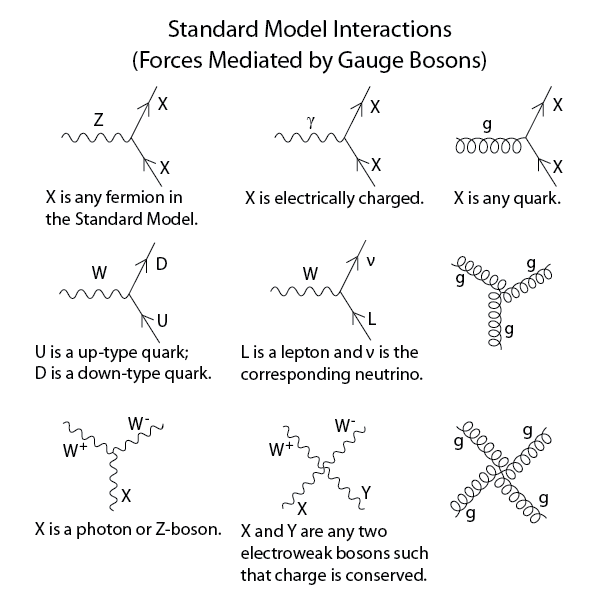
\includegraphics[width=.9\linewidth]{Standard_Model_Feynman_Diagram_Vertices}
\end{figure}

We briefly overview the entirety of the fundamental interactions of the Standard Model; these can also be found in \ref{fig:sm_interactions}.

The electromagnetic force, mediated by the photon, interacts with via a three-point coupling all charged particles in the Standard Model.
The photon thus interacts with all the quarks, the charged leptons, and the charged $W^\pm$ bosons.

The weak force is mediated by three particles : the $W^\pm$ and the $Z^0$.
The $Z^0$ can interacts with all fermions via a three-point coupling.
A real $Z_0$ can thus decay to a fermion-antifermion pair of all SM fermions except the top quark, due to its large mass.
The $W^\pm$ has two important three-point interactions with fermions.
First, the $W^\pm$ can interact with an up-like quark and a down-like quark; an important example in LHC experiments is $t \rightarrow Wb$
The coupling constants for these interactions are encoded in the unitary matrix known as the Cabibbo–Kobayashi–Maskawa (CKM) matrix \cite{Cabibbo:1963yz,Kobayashi:1973fv}, and are generally known as flavor-changing interactions.
Secondly, the $W^\pm$ interacts with a charged lepton and its corresponding neutrino.
In this case, the unitary matrix that corresponds to CKM matrix for quarks is the identity matrix, which forbids (fundamental) vertices such as $\mu \rightarrow We$.
For leptons, instead this is a two-step process : $\mu \rightarrow \nu_mu W \rightarrow \nu_mu \bar{\nu_e} e$.
Finally, there are the self-interactions of the weak gauge bosons.
There is a three-point and four-point interaction; all combinations are allowed which conserve electric charge.

The strong force is mediated by the gluon, which as discussed above also carries the strong color charge.
There is the fundamental three-point interaction, where a quark radiates a gluon.
Additionally, there are the three-point and four-point gluon-only interactions.

\section{Deficiencies of the Standard Model}

At this point, it is quite easy to simply rest on our laurels.
This relatively simple theory is capable of explaining a very wide range of phenomenom, which ultimately break down only to combinations of nine diagrams shown in Fig.\ref{fig:sm_interactions}.
Unfortunately, there are some unexplained problems with the Standard Model.
We cannot go through all of the potential issues in this thesis, but we will motivate the primary issues which naturally lead one to \textit{supersymmetry}, as we will see in Ch.\ref{ch:susy}.

The Standard Model has many free paramaters; see Table \ref{tab:sm_free_parameters}
\begin{table}
\centering
\caption{Parameters of the Standard Model.  For values dependent on the renormalization scheme, we use a combination of the on-shell normalization scheme \cite{Hollik:1988ii, Bardin:1989vz, Kennedy:1988rt, Sirlin:1980nh} and  modified minimal subtraction scheme with $m_{\bar{MS}}$ as indicated in the table\cite{ Fanchiotti:1992tu}}.
\label{tab:sm_free_parameters}
\begin{tabular}{| l | l | l |}
\hline
$m_e$             & Electron mass                  & 511 keV                           \\ \hline
$m_\mu$           & Muon mass                      & 105.7 MeV                         \\ \hline
$m_\tau$          & Tau mass                       & 1.78 GeV                          \\ \hline
$m_u$             & Up quark mass                  & 1.9 MeV   ($m_{\bar{MS}} = 2 GeV$)                        \\ \hline
$m_d$             & Down quark mass                & 4.4 MeV   ($m_{\bar{MS}} = 2 GeV$)                       \\ \hline
$m_s$             & Strange quark mass             & 87 MeV    ($m_{\bar{MS}} = 2 GeV$)                        \\ \hline
$m_c$             & Charm quark mass               & 1.32 GeV  ($m_{\bar{MS}} = m_c$)                        \\ \hline
$m_b$             & Bottom quark mass              & 4.24 GeV  ($m_{\bar{MS}} = m_b$)  \\ \hline
$m_t$             & Top quark mass                 & 172.7 GeV (on-shell renormalization)                       \\ \hline
$\theta_{12}$ CKM & 12-mixing angle                & 13.1$^{\circ}$                    \\ \hline
$\theta_{23}$ CKM & 23-mixing angle                & 2.4$^{\circ}$                     \\ \hline
$\theta_{13}$ CKM & 13-mixing angle                & 0.2$^{\circ}$                     \\ \hline
$\delta$ CKM      & CP-violating Phase             & 0.995                             \\ \hline
$g'$              & U(1) gauge coupling            & 0.357     ($m_{\bar{MS}} = m_Z$)                         \\ \hline
$g$               & SU(2) gauge coupling           & 0.652     ($m_{\bar{MS}} = m_Z$)                         \\ \hline
$g_s$             & SU(3) gauge coupling           & 1.221     ($m_{\bar{MS}} = m_Z$)                         \\ \hline
$\theta{QCD}$     & QCD vacuum angle               & \order 0                          \\ \hline
VEV               & Higgs vacuum expectation value & 246 GeV                           \\ \hline
$m_H$             & Higgs mass                     & 125 GeV                           \\ \hline
\end{tabular}
\end{table}
In general, we prefer models with less free parameters.
A great example of this fact, and the primary experimental evidence for EWSB, is the relationship between the couplings of the weak force and the masses of the gauge bosons of the weak force :
\begin{equation}
\rho \equiv \frac{m_W^2}{m_Z^2 \cos^2 \theta_W } \stackrel{?}{=} 1
\end{equation}
where $?$ indicates that this is a testable prediction of the Standard Model (in particular, that the gauge bosons gain mass through EWSB).
This relationship has been measured  within experimental and theoretical predictions.
We would like to produce additional such relationships, which would exist if the Standard Model is a low-energy approximation of some other theory.

An additional issue is the lack of \textit{gauge coupling unification}.
The couplings of any quantum field theory ``run'' as a function of the distance scales (or inversely, energy scales) of the theory.
The idea is closely related to the unification of the electromagnetic and weak forces at the so-called \textit{electroweak scale} of $O(100 \GeV)$.
One would hope this behavior was repeated between the electroweak forces and the strong force at some suitable energy scale.
\begin{figure}
\caption{The running of Standard Model gauge couplings.  The Standard Model couplings do not unify at high energies, which indicates it cannot completely describe nature through the Planck scale.} \label{fig:sm_gauge_coupling}
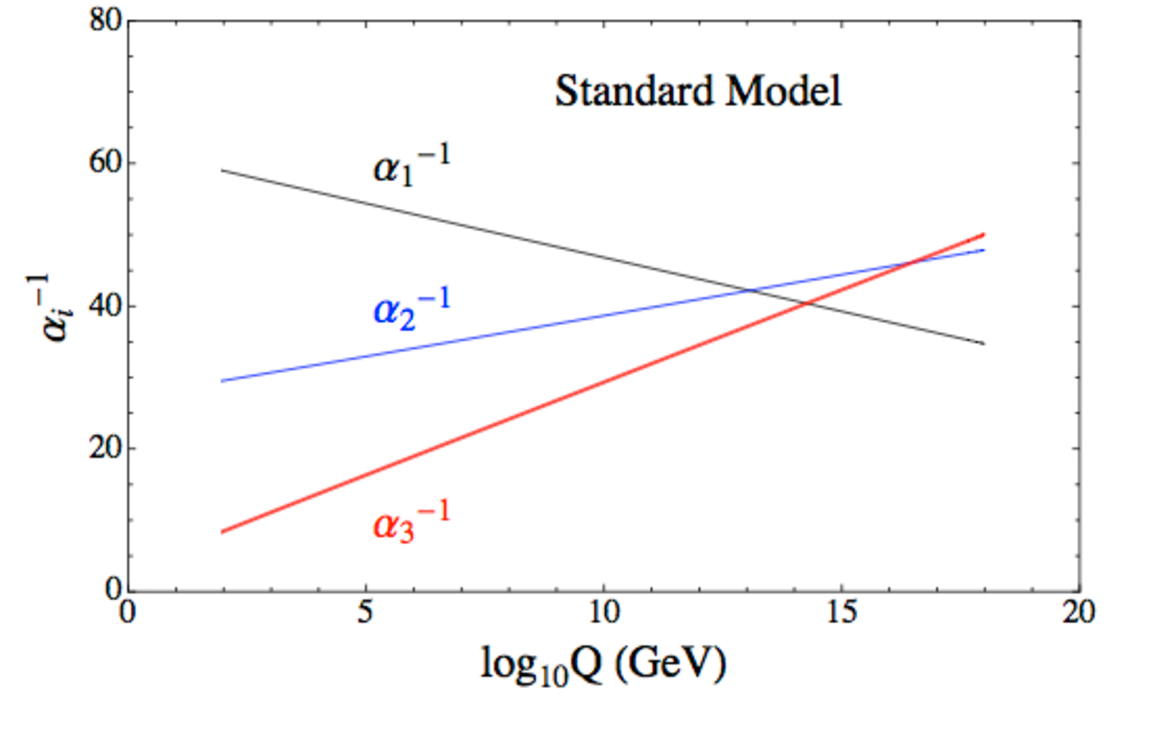
\includegraphics[width=.9\linewidth]{Grand_unification_couplings_sm}
\end{figure}
The Standard Model does automatically not exhibit this behavior, as we can see in Fig.\ref{fig:sm_gauge_coupling}.

\begin{figure}
\caption{The dominant quantum loop correction to the Higgs mass in the Standard Model.} \label{fig:sm_higgs_corrections}
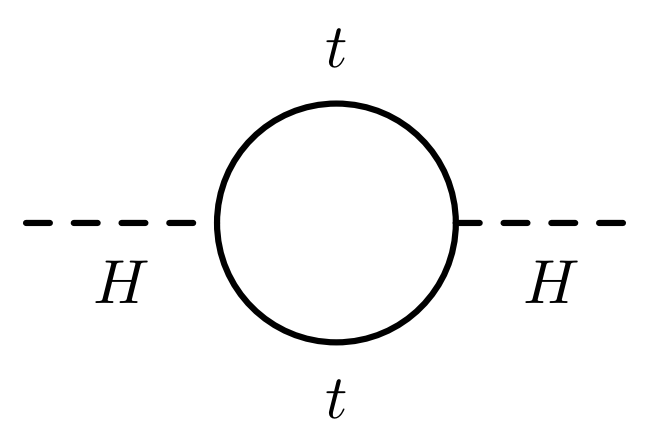
\includegraphics[width=.9\linewidth]{sm_higgs_corrections}
\end{figure}
The most significant problem with the Standard Model is the \textit{hierarchy problem}.
In its most straightforward incarnation, the Higgs scalar field is subject to quantum corrections through loop diagrams, as shown in Fig.\ref{fig:sm_higgs_corrections}.
For demonstration, we use the contributions from the top quark, since the top quark has the largest Higgs Yukawa coupling due to its large mass.
In general, we should expect these corrections to quadratically dependent on the scale of the ultraviolet physics, $\Lambda$.
Briefly assume there is no new physics before the Planck scale of gravity, $\Lambda_{\text{Planck}} = 10^{19} \GeV$.
In this case, we expect the corrections to the Higgs mass like
\begin{equation}
\delta m^2_H \approx \begin{pmatrix} \frac{m_t}{8\pi^2 <\phi>_{VEV}} \end{pmatrix}^2 \Lambda_{Planck}^2.
\end{equation}
To achieve the miraculous cancellation required to get the observed Higgs mass of 125 \GeV, one needs to then set the bare Higgs mass $m_0$, our input to the Standard Model Lagrangian, itself to a \textit{precise} value $\order 10^{19} \GeV$.
This extraordinary level of parameter finetuning is quite undesirable, and within the framework of the Standard Model, there is little that can be done to alleviate this issue.

An additional concern, of a different nature, is the lack of a \textit{dark matter} candidate in the Standard Model.
Dark matter was discovered by observing galactic rotation curves, which showed that much of the matter that interacted gravitionally was invisible to our (electromagnetic) telescopes \cite{Rubin:1970zza, Roberts:1970zza, Rubin:1980zd, Rubin:1985ze, Bosma:1981zz, Persic:1995ru, darkMatterPrimer}.
The postulation of the existence of dark matter, which interacts at least through gravity, allows one to understand these galatic rotation curves.
Unfortunately, no particle in the Standard Model could possibly be the dark matter particle.
The only candidate truly worth another look is the neutrino, but it has been shown that the neutrino content of the universe is simply too small to explain the galatic rotation curves \cite{Quigg:2008ab, darkMatterPrimer}.
The experimental evidence from the galactic rotations curves thus show there \textit{must} be additional physics beyond the Standard Model, which is yet to be understood.

In the next chapter, we will see how these problems can be alleviated by the theory of supersymmetry.

\begin{figure}
\caption{Particles of the Standard Model} \label{fig:sm_particles}
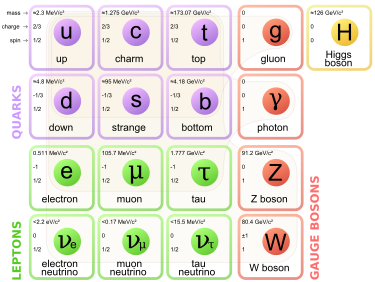
\includegraphics[width=.9\linewidth]{Standard_Model_of_Elementary_Particles}
\end{figure}

% \subsection{$\Lagr_{\psi}$ }

% We cannot write down any mass terms for fermions in the Standard Model.
% Dirac mass terms are forbidden since they are all assigned to ``chiral'' representations of the gauge symmetry.
% Majorana mass terms are disallowed since there are no fields with $Y \slashed{=} 0$.

% \subsection{$\Lagr_{Yuk}$ }

% We write the Yukawa portion of the Standard Model Lagrangian

% \begin{equation}
% \Lagr_{Yuk} = Y_{ij}\bar{L_{Li} E_{Rj}} \phi + h.c.
% \end{equation}

% The Yukawa matrix $Y$ is a general complex 3 $\times$ 3 matrix of dimensionless couplings which can be diagonalized, leading to a diagonal matrix with only three real parameters $(y_e , y_\mu , y_\tau)$.
% This reflects the fact that for the electron, muon, and tau lepton, the interaction basis is the same as the mass basis; this is the same as saying an electron has a well-defined mass.

% \section{$\Lagr_\phi$, Electroweak Symmetry breaking and the Higgs Boson}

% Let us now recall that local gauge invariance means that the vector fields in this theory are \textit{massless}.
% N\"aively, it seems this combined with the chirality of the Standard Model, that \textit{none} of the fields have masses.
% The solution to this seeming conundrum is of course the well-known ``Higgs'' mechanism, described in Sec. \ref{subsec:symmetry_breaking}.

% In the Standard Model, the Higgs potential is given by
% \begin{equation} \label{eq:higgs_potential}
% \Lagr_\phi = -\mu^2 \phi^\dagger \phi - \lambda (\phi^\dagger \phi)^2.
% \end{equation}

% Since $\lambda$ is dimensionless and real, to have a potential bounded from below, we require $\lambda > 0$.
% To break the gauge symmetry, we require $\mu^2 < 0$, leading again to the sombrero potential \ref{fig:sombrero}.
% We define
% \begin{equation}
% v^2 = - \frac{\mu^2}{\lambda}.
% \end{equation}

% This allows us to write \ref{eq:higgs_potential} as
% \begin{equation} \label{eq:higgs_potential_rewritten}
% \Lagr_\phi = - \lambda (\phi^\dagger \phi - \frac{v^2}{2})^2
% \end{equation}
% after dropping the constant term.

% This means the $\phi$ field acquires a VEV $|<\phi>| = v/\sqrt{2}$.
% Choosing the convenient gauge
% \begin{equation}
% \phi = \begin{pmatrix} 0 \\ v/\sqrt{2} \end{pmatrix},
% \end{equation}

% The VEV breaks the $SU(2)_L \otimes U(1)_Y$ symmetry to a $U(1)_{EM}$ subgroup.
% We can identify the unbroken generator of this $U(1)_{EM}$ subgroup as $Q_{EM} = T_3 + Y/2$, since this vanishes in the down component
% \begin{equation}
% Q_{\gamma} \phi = (T_3 + Y/2) \phi = (\frac{1}{2} \sigmathree + \frac{1}{2} I ) \begin{pmatrix} 0 \\ v/\sqrt{2} \end{pmatrix}.
% \end{equation}
% Here we see the indicative $\gamma$ for the photon, as this unbroken $U(1)_{EM}$ symmetry is of course the symmetry associated to the electromagnetic force mediated by the gauge boson known as the photon.

% There are three broken generators : $T_1, T_2, T_3 - Y/2$.
% These are each associated to one of the massive gauge bosons induced by the symmetry breaking.
% Choosing a gauge which rotates away the ``eaten'' Goldstone boson degrees of freedom, we can write the Higgs field as
% \begin{equation}
% \label{eq:higgs_field}
% \phi = \frac{1}{\sqrt{2}}\begin{pmatrix} 0 \\ v + h(x) \end{pmatrix}.
% \end{equation}

% \section{Particle Spectrum : Standard Model Lagrangian after Electroweak Symmetry Breaking}

% We can now return to the Standard Model Lagrangian and use the equation for the Higgs field after EWSB \ref{eq:higgs_field}.
% This will show us the ``physical'' particle content of the Standard Model.

% \subsection{Particle content associated to $\Lagr_\phi$}

% Setting $phi$ as in Eq.\ref{eq:higgs_field}, we quickly see that we can rewrite Eq.\ref{eq:higgs_potential_rewritten} as
% \todo{ CHECK FACTORS OF TWO}
% \begin{equation}
% \Lagr_\phi = - \lambda (\phi^\dagger \phi - \frac{v^2}{2})^2  = - \lambda ( \frac{1}{2} (v + h(x))^2 - \frac{v^2}{2})^2 = - \lambda ( h(x)^2 + vh(x))^2 = -\lambda ( h(x)^4 + v h(x)^3 + \frac{v^2}{2} h(x)^2 ).
% \end{equation}

% Interpreting the Higgs field squared term as the mass term of the Higgs boson, we see that $m_H = \sqrt{2 \lambda} v$.

% \subsection{Particle content associated to $\Lagr_{kin}$}

% Again using Eq.\ref{eq:higgs_field} and $\Dmuup = \dmuup + ig_s G^\mu_a L_a + i g W^\mu_a T_a + i g' Y B^\mu $, we can see how the mass terms associated to the three massive gauge bosons, and also see how the photon stays massless.
% The mass terms for the gauge boson fields come from the kinetic term of the Higgs field :
% For each of the vector boson fields, we have the follow field strengths :

% \begin{equation}
% \begin{align}
% G^{\mu\nu}_a = \dmuup G^\nu_a + \partial^\nu G^\mu_a - g_s f_{abc} G^\mu_b G^\nu_c \\
% W^{\mu\nu}_a = \dmuup W^\nu_a + \partial^\nu W^\mu_a - g \epsilon_{abc} W_b^\mu W_c^\nu \\
% B^{\mu\nu}   = \dmuup B^\nu   + \partial^\nu B^\mu
% \end{align}
% \end{equation}

% where $g$ and $g_s$ are the electroweak and strong coupling constant.

% We can write the covariant derivative for the Standard Model as
% \begin{equation}
% \Dmuup = \dmuup + ig_s G^\mu_a L_a + i g W^\mu_a T_a + i g' Y B^\mu
% \end{equation}
% where $L_a$ and $T_a$ are the generators of $SU(3)_C $ and $SU(2)_L$ respectively for each of the representations.
% Explicitly, for the $SU(3)_C$ triplets, $L_a = \frac{1}{2} \lambda_a$ and for the $SU(3)_C$ singlets, $L_a = 0$. \todo{GELLMANN and Pauli matrices}.
% For $SU(2)_L$ doublets, $T_a = \frac{1}{2} \sigma_a $ and for $SU(2)_L$ singlets, $T_a = 0$.

% The combination of these terms allows us to write the kinetic terms of the Lagrangian as
% \begin{equation}
% \begin{align}
% \Lagr_{kin} = G^{\mu\nu} G_{\mu\nu} + W^{\mu\nu} W_{\mu\nu} + B^{\mu\nu} B_{\mu\nu}\\
%  + \Dmuup Q_L \Dmu Q_L + \Dmuup U_R \Dmu U_R +  \Dmuup D_R \Dmu D_R + \Dmuup L_L \Dmu L_LL + \Dmuup E_R \Dmu E_R
% \end{align}
% \end{equation}
